\hypertarget{ch4}{%
\chapter{Towards a multisensor optical-radar approach for snow water equivalent retrievals}\label{ch4}}

%==============================================================================
%==============================================================================
%==============================================================================

\hypertarget{ch4-abstract}{\section{Abstract}\label{ch4-abstract}}


%==============================================================================
%==============================================================================
%==============================================================================
\hypertarget{ch4-intro}{\section{Introduction}\label{ch4-intro}}



Measuring the spatial and temporal distribution of snow water equivalent (SWE) and snow depth in the world’s mountains is the preeminent unsolved challenge facing snow hydrology \citep{dozierEstimatingSpatialDistribution2016}. Despite the critical importance of these measurements, no single spaceborne sensor will be able to monitor SWE from all snow classes \citep{sturmSeasonalSnowCover1995, sturmRevisitingGlobalSeasonal2021} globally at scales relevant to basin-scale water resource management \citep{lettenmaierInroadsRemoteSensing2015}. Thus, breakthroughs in spaceborne SWE monitoring will require a multisensor approach \citep{durandAchievingBreakthroughsGlobal2021}, also known as sensor fusion, with the combination of optical and Synthetic Aperture Radar (SAR) as a prime candidate. 

SAR will be at the forefront of future advancements in satellite remote sensing of SWE and snow depth, with multiple snow-focused SAR missions under development from NASA and the Canadian Space Agency (CSA) \citep{tsangReviewArticleGlobal2022, yuehSatelliteSyntheticAperture2021, garnaudQuantifyingSnowMass2019}. In addition, there are planned launches of L-band SARs such as the NASA-ISRO SAR (NISAR) in 2024 and the European Space Agencies (ESA) Radar Observation System for Europe in L-band (ROSE-L) near the end of the decade. Various recent studies have forwarded our abilities in using L-band interferometric SAR (InSAR) for SWE change monitoring in preparation for the impending NISAR and ROSE-L launches \citep{tarriconeEstimatingSnowAccumulation2023a, marshallLBandInSARDepth2021, naglerAirborneExperimentInsar2022}. Moreover, the launch of Sentinel-1C in 2023 will reestablish the two-satellite constellation and continue global C-band coverage, broadening the spaceborne SAR options. 

%%%%: topic: reviewing SAR-based dry snow cover algorithms and showing they're not sufficient
Snowpack that is important for human water resources mainly exists in complex mid-latitude mountain environments (cite). In the WUS, snow covered area (SCA) ranges between a median value of $\sim$3,000 km$^{2}$ at its summer minimum and $\sim$10$^{6}$ km$^{2}$ during the winter maximum \citep{rittgerSnowToday2022} (more here, possibly percentage of land area). Existing SAR-based techniques do not possess the capability to accurately delineate dry snow cover on their own \citep{tsaiRemoteSensingSnow2019}. There have been experimental attempts to use SAR at various frequencies and polarizations to detect dry snow \citep{rottThematicStudiesAlpine1994, shiMappingSeasonalSnow1997}. More recent studies employed a complex polarimetric decomposition \cite{varadeIdentificationSnowUsing2020} or machine learning techniques \cite{tsaiWetDrySnow2019}. While there has been progress in this area, none of these methods are mature enough for operational snow cover mapping. \par

%%%% topic: a review of current operational snow cover products
Contrarily, methods for passive microwave (PM), optical, and near-infrared (NIR) snow cover mapping are mature and routinely practiced \citep{dozierMultispectralHyperspectralRemote2004,saberiReviewSnowWater2020}. PM instruments produce data on the spatial scale of tens of kilometers, are only effective in dry snowpacks $<$~1 m, and therefore are not suitable for mountain watershed snowpack applications \citep{takalaEstimatingNorthernHemisphere2011a,pulliainenPatternsTrendsNorthern2020}. Optical and NIR snow mapping methods date back to the earliest earth-observing satellites \citep{rangoSatellitePotentialsSnowcover1976a}. Numerous studies have utilized multi-spectral data in mountain environments from the Landsat~5--9 \citep{dozierSpectralSignatureAlpine1989} and the Moderate Resolution Imaging Spectroradiometer (MODIS) \citep{painterRetrievalSubpixelSnowcovered2003, painterRetrievalSubpixelSnow2009, rittgerAssessmentMethodsMapping2013}. 

These optical methods are the basis for various snow cover products. In the western US (WUS), there is a fractional snow covered area (fSCA) product from Landsat~8/9 \citep{selkowitzUSGSLandsatSnow2017}, and a Normalized Snow Difference Index (NDSI) \citep{dozierSpectralSignatureAlpine1989, hallDevelopmentMethodsMapping1995} product from the MODIS \citep{hallMODISSnowcoverProducts2002} and the Visible Infrared Imaging Radiometer Suite (VIIRS) \citep{justiceLandCryosphereProducts2013}. For Europe and various other parts of the world, \cite{gascoinTheiaSnowCollection2019a} created the Theia Snow collection, which uses Landsat~8 and Sentinel~2A/B independently to map binary snow presence.

%%%% topic: lidar from space won't work
Previous research has explored different combinations of multisensor approaches for different snow monitoring applications. The Airborne Snow Observatory (ASO) \citep{painterAirborneSnowObservatory2016} leverages suborbital lidar altimetry \citep{deemsLidarMeasurementSnow2013}, hyperspectral imaging \citep{nolinMappingAlpineSnow1993}, and spatially distributed snow density modeling \citep{marksSpatiallyDistributedEnergy1999,hedrickDirectInsertionNASA2018,meyerOperationalWaterForecast2023a} to estimate basin-scale SWE at fine resolutions (1--50~m). While this technique is now operational, there is no clear pathway to space for spatially distributed lidar retrievals. Currently, only linear transects from satellites such as NASA's Ice, Cloud and Land Elevation Satellite-2 (ICESat-2) \citep{abdalatiICESat2LaserAltimetry2010} and the Global Ecosystem Dynamics Investigation (GEDI) \citep{dubayahGlobalEcosystemDynamics2020} are possible. Moreover, even the sparse measurements from the aforementioned spaceborne lidars show uncertainties of 1--2~m for snow depth retrievals in complex terrain \citep{enderlinUncertaintyICESat2ATL062022, deschamps-bergerEvaluationSnowDepth2022}. 

%%%% topic: optical fusion
% *** Recently, NASA released the Harmonized Landsat and Sentinel-2 (HLS) data product which fuses the two sensors to produce lower temporal resolution surface reflectance data. Rittger et al. \citep{rittgerMultisensorFusionUsing2021} combined Landsat and MODIS with machine learning to achieve a spatiotemporally complete 30 m fSCA dataset over the Sierra Nevada Mountains, CA. ****

%%
% Recently, \cite{stillingerLandsatMODISVIIRS2023a} performed an uncertainty analysis of various fSCA products from MODIS, VIIRS, and Landsat using airborne lidar-based fSCA as validation. They found some variability in the fSCA products, with the spectrally unmixed data performing better, but overall modest differences. \cite{bairHowTradeoffsSatellite2023}


%%%% topic: SAR/optical for SWE or depth fusion products
Few studies have employed optical and SAR data synergistically for snow depth and SWE retrievals. \cite{lievensSnowDepthVariability2019,lievensSentinel1SnowDepth2022} developed a Sentinel-1 C-band snow depth retrieval algorithm using the co-polarized and cross-polarized backscatter ratio. They identified snow cover using 1 km$^{2}$ binary snow cover information from the Interactive Multisensor Snow and Ice Mapping System (IMS) \citep{u.s.nationalicecenterIMSDailyNorthern2008, ramsayInteractiveMultisensorSnow1998, helfrichEnhancementsForthcomingDevelopments2007}, and fractional forest cover using the 1~km$^{2}$ global consensus land cover dataset \citep{tuanmuGlobal1kmConsensus2014}, at both European and Northern Hemispherical scales. These new methods are promising, especially as the physical mechanisms governing the C-band retrievals continue to emerge \citep{zhuModelingScatteringDense2023}. \cite{tarriconeEstimatingSnowAccumulation2023a} utilized Landsat fSCA information with UAVSAR \citep{hensleyUAVSARInstrumentDescription2008} L-band InSAR data to estimate both snow ablation and accumulation in the Jemez Mountains, NM. They note the multifaceted importance of an optical-radar multisensor approach for snow cover delineation and SAR atmospheric correction. 

These past studies have subjectively selected various products (e.g., fSCA, binary, NSDI), spatial resolutions ($\sim$ 1--1000 m), and temporal resolutions (1--16~d) without any systematic investigation of the uncertainties associated with each. Our study aims to better understand the variability between common snow cover data products and how that uncertainty propagates into SAR-based SWE retrieval techniques. To do this, we analyze L-band InSAR SWE changes estimates from UAVSAR collected by the NASA SnowEx 2020 \cite{marshallNASASnowEx20202019} campaign in the Upper San Joaquin River basin (USJ) in Sierra Nevada Mountains, CA. NISAR's launch in early 2024 makes the InSAR-based approach the most time-sensitive of the SWE measurement techniques.

% -Despite the previously stated importance of a multisensor snow depth and SWE monitoring approach, few works have explored the best combination of sensors.
% - Herein, we will refer to our methodology as a ``multisensor" approach. Previous works (karl, add others) have used the term ``sensor fusion", which can be thought of as the same thing. Neither of these terms has concrete definitions, and therefore our word choice is subjective.


%==============================================================================
%%%%%%%%%%%%%%%%%%%%%%%%%%%%%%%%%%%%%%%%%%%%%%%%%%%%%%%%%%%%%%%%%%%%%%%%%%%%%%%%
\hypertarget{ch4-methods}{\section{Study area}\label{ch4-methods}}

The USJ is approximately 4244~km$^{2}$ in land area, spanning from the high-elevation Sierra peaks (4227~m) in the east to flat low-elevation (153~m) Central Valley in the west (Fig.~\ref{fig:multisensor_study_area}). The main channel flows into Millerton Lake, which is one of the largest reservoirs in the Central Valley. The USJ is mainly land cover is mainly various types of conifer species, except for the highest elevations. These areas are in the alpine with shrub-like or no vegetation. The UAVSAR flight line shown in red mainly exists with the USJ boundary but extends further to the north and south.

\begin{figure}[ht]
\includegraphics[width=\textwidth]{figures/ch4_figs/agu_map_v5.png}
\centering
\caption{Showing \textbf{(a)} elevation, \textbf{(b)} land cover, \textbf{(c)} canopy cover (\%) for the UAVSAR flight line (red) and the USJ basin (black).}
\label{fig:multisensor_study_area}
\end{figure}
\clearpage

%==============================================================================
%%%%%%%%%%%%%%%%%%%%%%%%%%%%%%%%%%%%%%%%%%%%%%%%%%%%%%%%%%%%%%%%%%%%%%%%%%%%%%%%
\hypertarget{ch4-methods}{\section{Methods \& data overview}\label{ch4-methods}}

In this section, we overview the UAVSAR InSAR data products, the six different snow cover products and how they are produced, and the in situ snowpack information used.

%==============================================================================
%%%%%%%%%%%%%%%%%%%%%%%%%%%%%%%%%%%%%%%%%%%%%%%%%%%%%%%%%%%%%%%%%%%%%%%%%%%%%%%%
\hypertarget{ch4-methods}{\section{Study area}\label{ch4-methods}}

The USJ is approximately 4244~km$^{2}$ in land area, spanning from the high-elevation Sierra peaks (4227~m) in the east to flat low-elevation (153~m) Central Valley in the west (Fig.~\ref{fig:multisensor_study_area}). The main channel flows into Millerton Lake, which is one of the largest reservoirs in the Central Valley. The USJ is mainly land cover is mainly various types of conifer species, except for the highest elevations. These areas are in the alpine with shrub-like or no vegetation. The UAVSAR flight line shown in red mainly exists with the USJ boundary but extends further to the north and south.

\begin{figure}[ht]
\includegraphics[width=\textwidth]{figures/ch4_figs/agu_map_v5.png}
\centering
\caption{Showing \textbf{(a)} elevation, \textbf{(b)} land cover, \textbf{(c)} canopy cover (\%) for the UAVSAR flight line (red) and the USJ basin (black).}
\label{fig:multisensor_study_area}
\end{figure}
\clearpage


%%%%%%%%%%%%%%%%%%%%%%%%%%%%%%%%%%%%%%%%%%%%%%%%%%%%%%%%%%%%%%%%%%%%%%%%%%%%%%%%
\hypertarget{ch4-methods-1}{\subsection{UAVSAR}\label{ch4-methods-1}}

UAVSAR flights occurred on 26 February 2020 and 11 March 2020 and covered an area of $\sim$1600 km$^{2}$. These data were processed by the UAVSAR team at NASA's Jet Propulsion Laboratory (JPL) to create a single 14 d baseline 6 m ground projected InSAR pair. These products include unwrapped phase (herein, phase), coherence, and incidence angle ($\theta$). Table \ref{tab:uavsar_specs} shows the information on the radar (top) and the specific processing parameters (bottom). To better replicate the NISAR returns, we resampled the 6~m UAVSAR data to 80~m, which is the resolution NISAR data products will be produced. To do this, we used Sentinel-1 Geocoded Unwrapped Interferograms (S1 GUNW), which are produced in the same data format and spatial resolution (80 m) that NISAR data will be. These data are generated by NASA's Advanced Rapid Imaging and Analysis (ARIA) \citep{bekaertDevelopmentDisseminationStandardized2019,buzzangaSustainedMonitoringSubsidence2020} project and accessed via the Alaska Satellite Facility Distributed Active Archive Center (ASF DAAC).


\begin{figure}[ht]
\includegraphics[width=13cm]{figures/ch4_figs/data_section_plot_v3.png}
\centering
\caption{UAVSAR \textbf{(a)} coherence, \textbf{(b)} phase, \textbf{(c)} incidence angle from the 2/26--3/11 InSAR pair. The grey pixels in \textbf{(b)} are pixels lost in the unwrapping process, which is caused by low coherence values. The full extent of S1 GUNW \textbf{(d)} phase and \textbf{(e)} coherence from the 2/22--3/05 InSAR pair. The USJ watershed boundary and UAVSAR swath are shown by black lines, with Lake Tahoe represented by the blue in the top left corner. The black dotted line is a 1500 m contour approximating the seasonal snow zone.}
\label{fig:uavsar_cor_inc_phase_plot}
\end{figure}
\clearpage

\begin{table}[t]
\centering
\label{tab:uavsar_specs}
\caption{Technical specifications of the UAVSAR L-band radar (top). InSAR processing and data parameters of the 26 February--11 March UAVSAR InSAR pair (bottom).}
\begin{tabular}{ll}
\toprule Parameter & Value \\
\midrule
Wavelength & 23.84\,cm \\
Frequency & 1.26\,GHz \\
Polarization & Quad pol \\
Bandwidth & 80\,MHz \\
Pulse length & 40\,$\mu$s \\
Radar look direction & Left \\
Range swath width & 22\,km \\
Average near-range look angle & 28.01$^{\circ}$\\
Average far-range look angle & 68.9$^{\circ}$\\
\midrule
Native ground range pixel spacing & 6\,m \\
Number of looks in range & 3 \\
Number of looks in azimuth & 12 \\
Phase unwrapping method & ICU \\
Phase unwrapping filtering method & Low pass \\
Phase unwrapping filter window size & 3~pixels\,$\times$\,3~pixels \\
\bottomrule
\end{tabular}
\end{table}


%%%%%%%%%%%%%%%%%%%%%%%%%%%%%%%%%%%%%%%%%%%%%%%%%%%%%%%%%%%%%%%%%%%%%%%%%
\hypertarget{ch4-methods-2}{\subsection{Snow cover data}\label{ch4-methods-2}}

Optical snow cover information is traditionally derived using either the normalized snow difference index (NDSI) \citep{dozierSpectralSignatureAlpine1989} or spectral-mixture analysis \citep{rosenthalAutomatedMappingMontane1996,nolinMappingAlpineSnow1993}. While we provided a brief description of the methods below, the reader is referred to the aforementioned publications and \cite{stillingerLandsatMODISVIIRS2023} for a detailed description of the two techniques.

Snow is highly reflective in the visible (VIS) wavelengths ($\sim$0.4--0.7~$\mu$m) while demonstrating strong absorption characteristics in the shortwave infrared (SWIR) ($\sim$1--4~$\mu$m) spectrum. This relationship is leveraged by the NSDI equation:

\begin{equation}
\label{eq:ndsi}
NDSI = \frac{VIS - SWIR}{VIS + SWIR}
\end{equation}

\noindent where the NDSI values range from $-$1 to $+$1. The exact band and wavelength will vary by remote sensing platform. 

\begin{figure}[h]
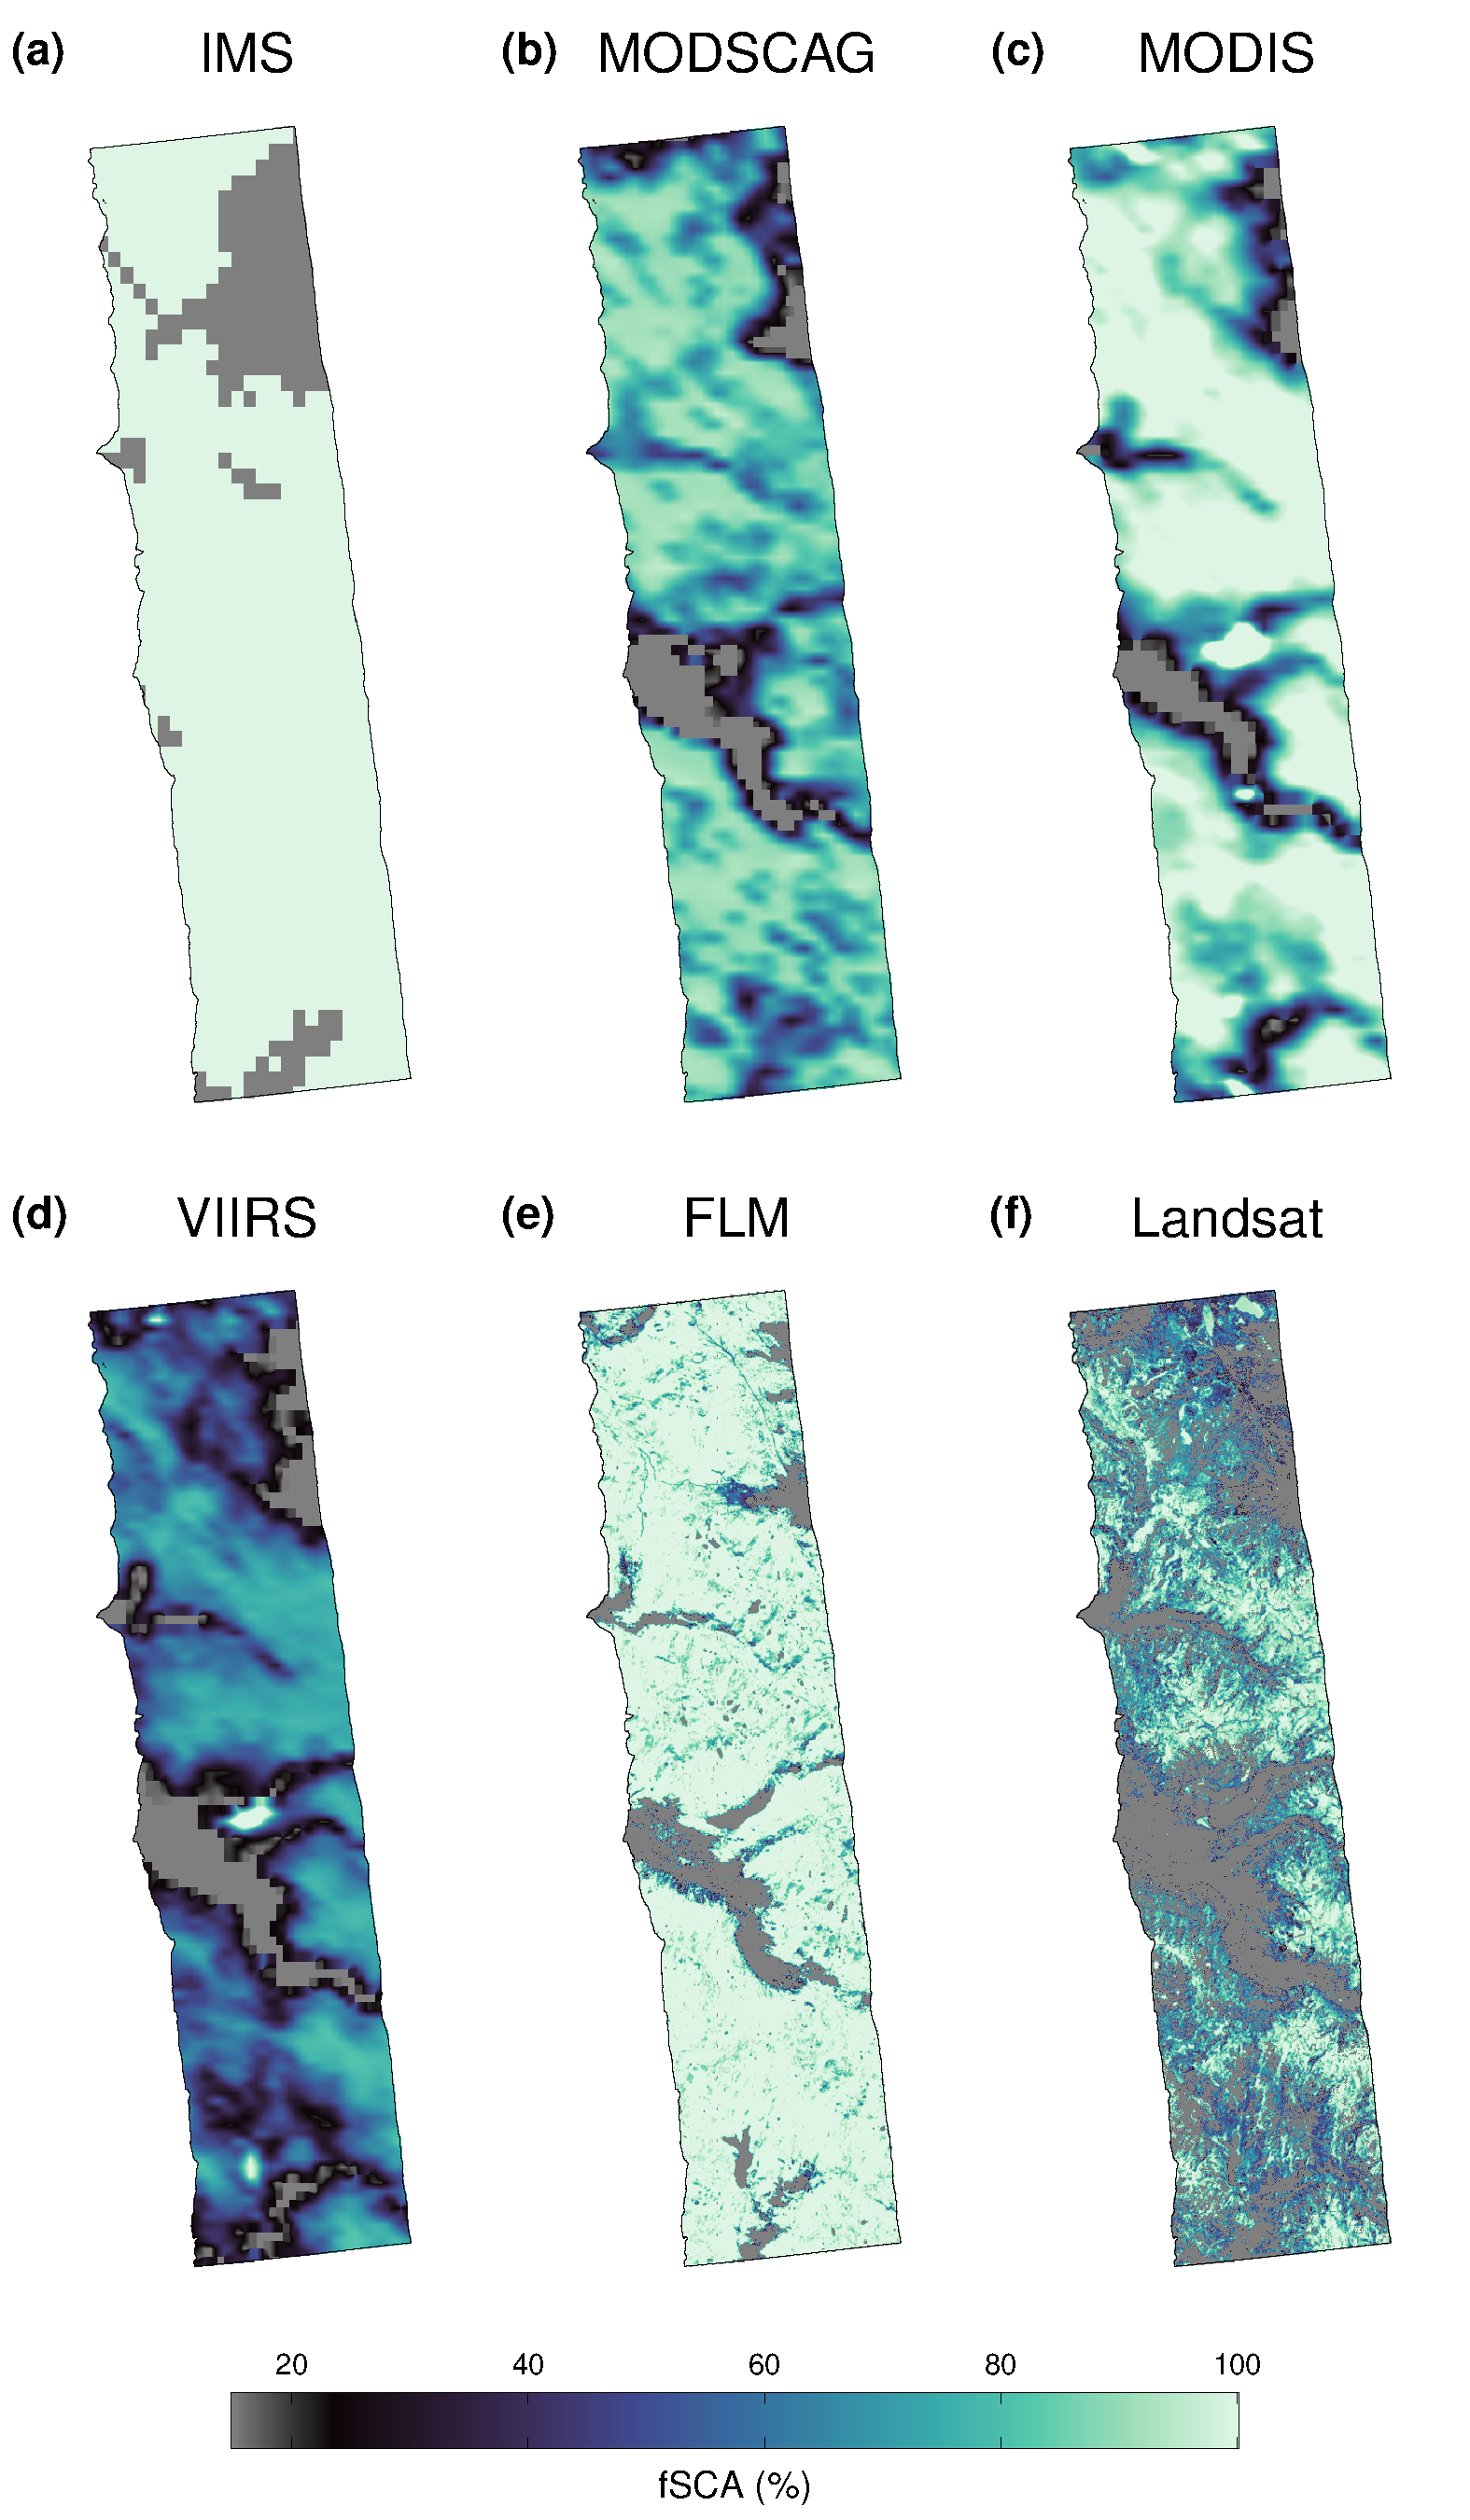
\includegraphics[width=\textwidth]{figures/ch4_figs/fsca_usvar_v2.pdf}
\caption{fSCA from \textbf{(a)} IMS, \textbf{(b)} MODSCAG, \textbf{(c)} MODIS, \textbf{(d)} VIIRS, \textbf{(e)} FLM, and \textbf{(f)} Landsat. The dark gray represents areas with < 15 \% fSCA}
\label{fig:fsca_plot}
\end{figure}

The data selected for our study have a range of spatial, temporal, and spectral resolutions. All data products in Fig.~\ref{fig:fsca_plot} were cropped and resampled to the 80~m NISAR resolution.  

\clearpage
%%%%%%%%%%%%%%%%%%%%%%%%%%%%%%%%%%%%%%%%%%%%%%%%%%%%%%%%%%%%%%%%%%%%%%%%%%%%%%%%
\hypertarget{ch4-methods-3}{\subsubsection{IMS}\label{ch4-methods-3}}

The National Oceanic and Atmospheric Administration’s National Environmental Satellite Data and Information Service (NOAA/NESDIS) Interactive Multisensor Snow and Ice Mapping System (IMS) is a hemispherical scale binary 1~km snow cover product (Fig.~\ref{fig:fsca_plot}a) originally created to help with numerical weather prediction 
\citep{ramsayInteractiveMultisensorSnow1998, helfrichEnhancementsForthcomingDevelopments2007}. The input data comes from a variety of platforms, including but not limited to: the National Oceanic and Atmospheric Administration's (NOAA's) next generation of geostationary satellites (GOES) constellation \citep{menzelIntroducingGOESIFirst1994}, the Advanced Very High Resolution Radiometer (AVHRR) \citep{cracknellAdvancedVeryHigh1997}, MODIS \citep{salomonsonMODISAdvancedFacility1989}, and the National Operational Hydrologic Remote Sensing Center (NOHRSC) SNOw Data Assimilation System (SNODAS) \citep{barrettandrewNationalOperationalHydrologic2003}.

%%%%%%%%%%%%%%%%%%%%%%%%%%%%%%%%%%%%%%%%%%%%%%%%%%%%%%%%%%%%%%%%%%%%%%%%%%%%%%%%
\hypertarget{ch4-methods-4}{\subsubsection{MODSCAG}\label{ch4-methods-4}}


The MODIS Snow-Covered Area and Grain size (MODSCAG) (Fig.~\ref{fig:fsca_plot}b) \citep{painterRetrievalSubpixelSnow2009} is a spectral-mixing model that uses various end-members (e.g., rock, soil, snow, clouds, etc.) to produce estimates of fSCA, fractional vegetation (fVEG), snow grain size, and albedo.

- add info here

%%%%%%%%%%%%%%%%%%%%%%%%%%%%%%%%%%%%%%%%%%%%%%%%%%%%%%%%%%%%%%%%%%%%%%%%%%%%%%%%
\hypertarget{ch4-methods-5}{\subsubsection{MODIS}\label{ch4-methods-5}}

The MODIS cloud-gap-filled (CGF) snow cover product \citep{hallEvaluationMODISVIIRS2019} provides daily NSDI values at 500Am spatial resolution from the Terra (MOD10A1F) and Aqua (MYD10A1F) satellites (Fig.~\ref{fig:fsca_plot}c) . These data account for cloud cover by excluding pixels flagged as clouds and refilling them with NDSI from the last cloud-free day. This process only goes on for eight days of cloud cover until the pixel is marked as NA. NDSI can be used to directly estimate fSCA \citep{salomonsonEstimatingFractionalSnow2004, salomonsonDevelopmentAquaMODIS2006,stillingerLandsatMODISVIIRS2023}. We estimated MODIS fSCA using the Eq.~\ref{eq:fsca}:

\begin{equation}
\text{fSCA} = 0.01 + (1.45 \times NDSI)
\label{eq:fsca}
\end{equation}


\hypertarget{ch4-methods-6}{\subsubsection{VIIRS}\label{ch4-methods-6}}

The Visible Infrared Imaging Radiometer Suite (VIIRS) on the Suomi National Polar Partnership (S-NPP) produces a daily CGF NDSI product (VNP10A1F) at 375~m spatial resolution (Fig.~\ref{fig:fsca_plot}d) \citep{hallEvaluationMODISVIIRS2019}. These data are generated and gap-filled using the same methods as the MODIS CFG data outlined in Section \ref{ch4-methods-5}. We converted the VIIRS NSDI values to fCSA using Eq. \ref{eq:fsca}.


\hypertarget{ch4-methods-7}{\subsubsection{FLM}\label{ch4-methods-7}}

The fused Landsat-MODIS (FLM) (Fig.~\ref{fig:fsca_plot}e)  fSCA product created by \cite{rittgerMultisensorFusionUsing2021} is spatiotemporally continuous 30~m over the Sierra Nevada, CA. The goal of their data fusion methods was to create a product with the high spatial resolution of Landsat (30~m) with the high temporal resolution of MODIS (1~d), leveraging the strengths of both sensors. These data were created using a combination of 170 Landsat scenes, daily MOD09GA Collection 6 in a sinusoidal projection at 463~m, physiographic information, spectral mixture algorithms, and random forest algorithm. 

\hypertarget{ch4-methods-8}{\subsubsection{Landsat fSCA}\label{ch4-methods-8}}

Landsat~8 fSCA (Fig.~\ref{fig:fsca_plot}f) \citep{selkowitzUSGSLandsatSnow2017} data are generated using a spectral unmixing analysis based on the MODSCAG algorithm developed for MODIS \citep{painterRetrievalSubpixelSnow2009}. The data processing workflow includes water masking, cloud masking, and canopy cover corrections \citep{selkowitzUSGSLandsatSnow2017, stillingerLandsatMODISVIIRS2023}. The data products include both viewable fSCA and total ground fSCA. To estimate total fSCA in areas with canopy cover, a moving window analysis algorithm is employed, and it selects.

\hypertarget{ch4-methods-8}{\subsection{In situ snow data}\label{ch4-methods-8}}

Snow pit from the SnowEx campaign
CADWR pillows -- name them

\hypertarget{ch4-methods-9}{\subsubsection{Canopy Cover}\label{ch4-methods-9}}

We used National Land Cover Database (NLCD) \citep{homerConterminousUnitedStates2020} canopy cover data. These data are Landsat-based 30~m native spatial resolution products that report canopy cover values in a percentage. These data are also used in the Landsat fSCA canopy cover correction.


%==============================================================================
%==============================================================================
%==============================================================================
\hypertarget{ch4-methods}{\section{Methods}\label{ch4-methods}}
\hypertarget{ch4-methods-1}{\subsection{Calculating InSAR $\Delta$SWE}\label{ch4-methods-1}}


First, the UAVSAR phase data were masked with each of the six fSCA products. A threshold of $>$\,15\,\% fSCA was set for a pixel to be considered snow covered. We then employ the InSAR $\Delta$SWE methodology described in Sec.~\ref{ch3-methods-1}. The SnowEx in situ data collection within the Sierra flight line did not include a permittivity measurement. Therefore, permittivity was estimated using the snow density to permittivity equation from \cite{guneriussenInSAREstimationChanges2001}:

\begin{equation}
\epsilon_\mathrm{s} = 1 + 1.6 * \rho_\mathrm{s} + 1.8 * \rho_\mathrm{s}^3
\label{eq:dens_to_perm}
\end{equation}


\noindent where snow permittivity is $\epsilon_\mathrm{s}$ and snow density is $\rho_\mathrm{s}$. Using Eq.~\ref{eq:insar_dswe}, pixel-wise $\Delta$SWE values were calculated with inputs of $\lambda$ (23.84\,cm), spatially distributed phase and $\theta$, $\rho_\mathrm{s}$ of 370~kg\,m$^{-3}$, and $\epsilon_\mathrm{s}$ of 1.68. 

To find the known change point to tether the initially relative InSAR $\Delta$SWE values, we used three snow pillows (vlc, mhp, ubc, wwc) from CADWR. The SnowEx $\Delta$SWE pit data could not be directly utilized as the phase values over the Mammoth CUES pit did not unwrap properly, resulting in the absence of any data. Additionally, the Panorama Dome pit was not dug during the study period. To account for uncertainties within the snow pillow geolocation, we extracted the UAVSAR pixel that the snow pillow was within and the eight surrounding pixels. We then took a spatial average of the relative InSAR $\Delta$SWE and the three pillows $\Delta$SWE values and subtracted them to obtain an absolute change. We report our volumetric $\Delta$SWE results in units of cubic decameters (dam$^{3}$). A cubic decameter is equal to 1000~m$^{3}$ or $\sim$0.81~acre-feet.

%==============================================================================
%==============================================================================
%==============================================================================
\hypertarget{ch4-methods-2}{\subsection{Quantifying $\Delta$SWE Variability}\label{ch4-methods-1}}

To understand how the various fSCA products impacted the scene wide $\Delta$SWE estimates, we performed a summing moving window analysis of the six UAVSAR-derived $\Delta$SWE datasets. The variability in the $\Delta$SWE data products solely comes from which pixels are considered snow covered and which are not. Therefore, a pixel-wise analysis is not an apt solution, as this would be comparing pixels with data to  NA (not available) values.

For the analysis, the $\Delta$SWE data were separated loss and gains to prevent the cancellation of patterns caused by opposite signs within an area. The pixel-wise SWE changes were then summed using a 41~$\times$~41 pixel moving window. Next, the standard deviation (SD) of the six moving window summed products was calculated. The relatively large window size was selected to minimize the of NA pixels in the SD calculation, where only datasets with 41-pixel squared areas of no snow will produced NA values. Summed pixels with NA values were not included in the SD calculations. We note the IMS data as the northeast corner has a large continuous swath of NA values.

\hypertarget{ch4-results}{\section{Results}\label{ch4-results}}
\hypertarget{ch4-results}{\subsection{$\Delta$SWE Estimates}\label{ch4-results}}

The spatially distributed 80~m UAVSAR $\Delta$SWE estimates for each of the six fSCA products are shown in Fig.~\ref{fig:uavsar_dswe}. The black areas represent pixels lost in the unwrapping process (Fig. \ref{fig:uavsar_cor_inc_phase_plot}b), and are static throughout Fig.~\ref{fig:uavsar_dswe}a--e. The gray area represents pixels not considered snow covered by the given fSCA product, and these areas spatially variable in the six scenes. Overall, the six scenes show a mean net SWE of $-$14,600~dam$^{3}$, with a mean gain of 3,100~dm$^{3}$ and loss of $-$17,800~dam$^{3}$ (Table~\ref{tab:dswe_stats}, Fig.~\ref{fig:dswe_bar_graph}). These values are consistent with in situ snow pillow data in this area, as there was a prolonged dry spell during 26 February to March 4 time span (***add appendix figure here).

\clearpage
\begin{figure}[t]
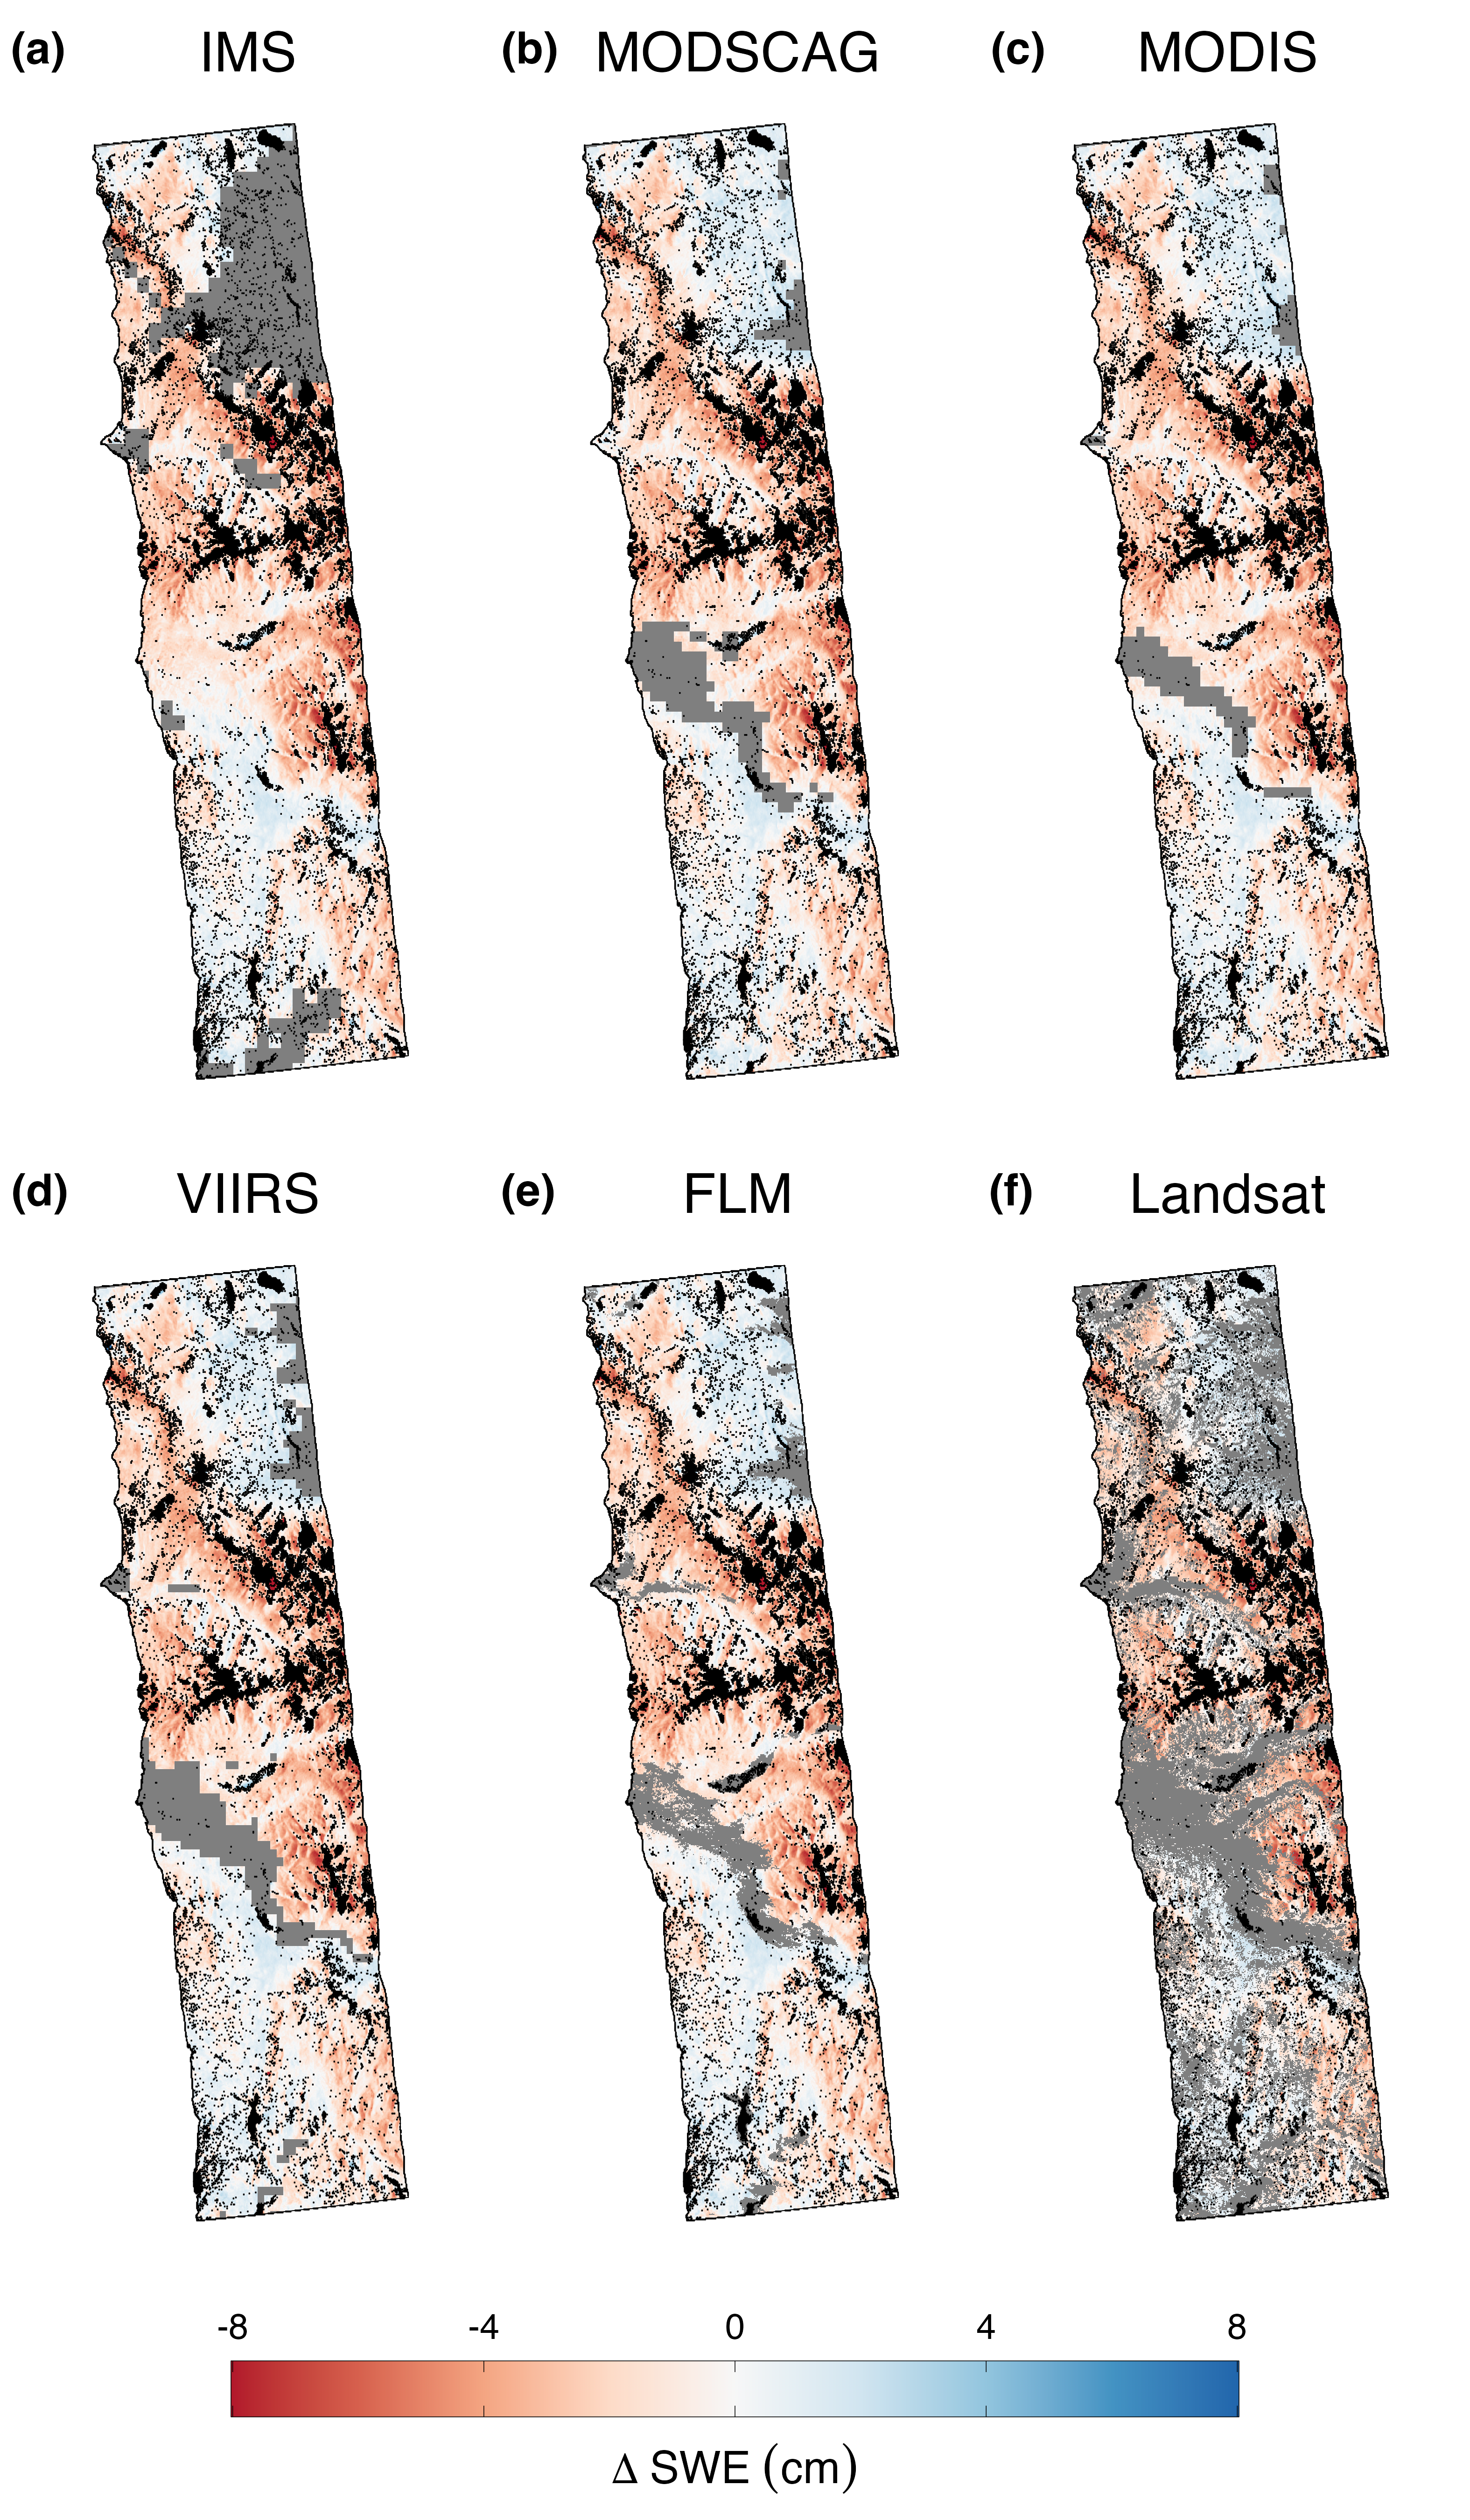
\includegraphics[width=\textwidth]{figures/ch4_figs/dswe_uavsar_v2.png}
\centering
\caption{UAVSAR InSAR derived $\Delta$SWE estimates with snow cover data from \textbf{(a)} IMS, \textbf{(b)} MODSCAG, \textbf{(c)} MODIS, \textbf{(d)} VIIRS, \textbf{(e)} FLM, and \textbf{(f)} Landsat. The dark gray represents areas with < 15 \% fSCA and the black represents pixels lost in the unwrapping process.}
\label{fig:uavsar_dswe}
\end{figure}

\clearpage
When disaggregated to SWE gains and losses, MODIS shows the greatest SWE gain of 3,800~dam$^{3}$. Landsat estimated the least (2,100~dam$^{3}$) with IMS showing a similar low value of 2,300~dam$^{3}$. The SWE gain values from MODSCAG, VIIRS, and FLM were quite similar to MODIS, with no product differing more than 400~dam$^{3}$.
MODIS also produced the greatest SWE loss ($-$19,100~dam$^{3}$), with Landsat again providing a low value of $-$12,900~dam$^{3}$. IMS, MODSCAG, VIIRS, and FLM again provided consistent estimates, with the standard deviation of these five data products SWE loss being only 350~dam$^{3}$. Landsat's SWE loss of $-$12,900~dam$^{3}$ is $-$5,800~dam$^{3}$ greater compared to the five other data products mean SWE loss of $-$18,700~dam$^{3}$. These differences propagate into the net $\Delta$SWE values, where the five products other than Landsat provided highly consistent values, with a mean net $\Delta$SWE $-$15,400~$\pm$~300~dam$^{3}$. We report a 35.1~\% difference between the aforementioned mean value and Landsat.


\begin{figure}[]
\centering
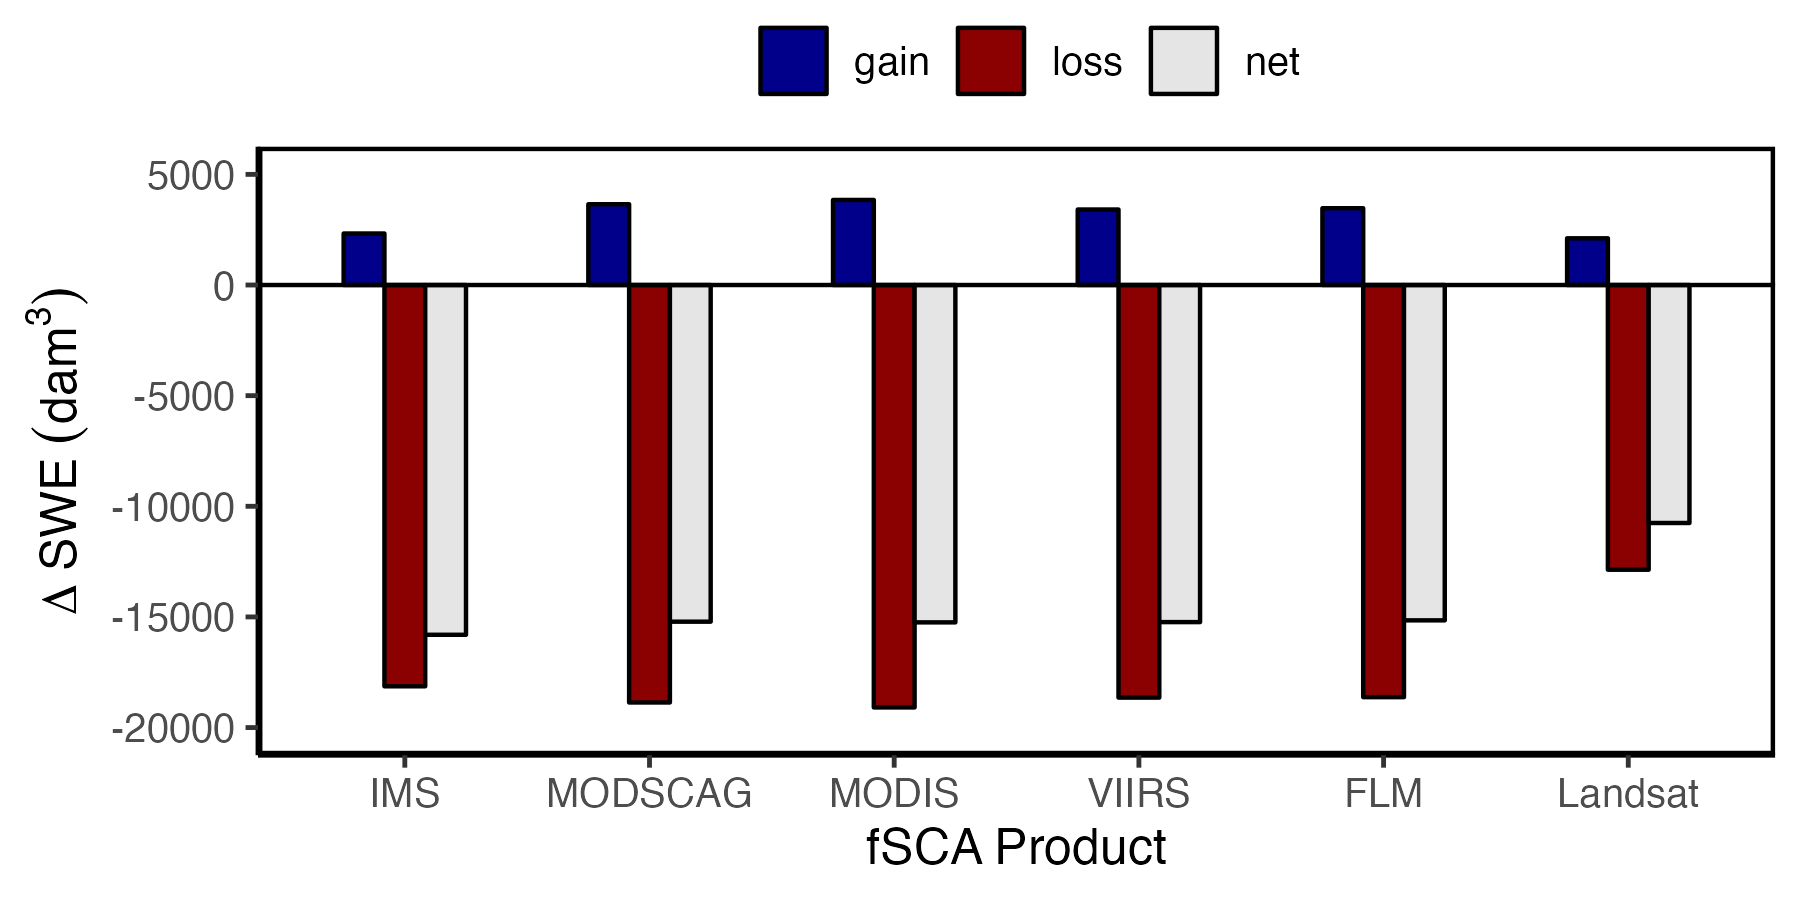
\includegraphics[width=\textwidth]{figures/ch4_figs/dswe_stats_dam3_v1.png}
\caption{Barplots of SWE gain, loss, and the net value for the six different fSCA products.}
\label{fig:dswe_bar_graph}
\end{figure}

\begin{table}
\centering
\caption{Displaying the total sum of $\Delta$SWE gains, losses, and overall net rounded to the nearest hundred for the six different fSCA products in Fig~\ref{fig:uavsar_dswe}.}
\begin{tabular}{lccc}
\toprule
& \multicolumn{3}{c}{$\Delta$SWE (dam$^{3}$)} \\
\midrule
fSCA Data & Gain & Loss & Net \\
\midrule
IMS & 2,300 & $-$18,200 & $-$15,900 \\
MODSCAG & 3,600 & $-$18,900 & $-$15,300 \\
MODIS & 3,800 & $-$19,100 & $-$15,300 \\
VIIRS & 3,400 & $-$18,700 & $-$15,300 \\
FLM & 3,400 & $-$18,700 & $-$15,200 \\
Landsat & 2,100 & $-$12,900 & $-$10,800 \\
\midrule
Mean & 3,100 & $-$17,800 & $-$14,600 \\
\bottomrule
\label{tab:dswe_stats}
\end{tabular}
\end{table}



\hypertarget{ch4-results}{\subsection{$\Delta$SWE Variability}\label{ch4-results}}

Fig.~\ref{fig:dswe_moving_window} shows the moving window sums of the $\Delta$SWE gains and losses. The majority of the SWE gains are recorded in the northeast and southeast portions of the swath. The SWE gain spatial patterns between the datasets are similar except for the northeast corner of the IMS data. This area is shown as no snow while MODSCAG, MODIS, VIIRS, and FLM display SWE gains on the order of 100--150~dam$^{3}$. Landsat shows SWE gain in this area as well but with a lesser magnitude of $\sim$50~dam$^{3}$. All datasets other than Landsat show consistent spatial patterns and SWE loss magnitudes. Landsat's spatial patterns are similar but with a lower amount of $\Delta$SWE. This is driven by Landsat's fSCA data not being as temporally continuous. The large area of NA values in the IMS data is not of concern as this area was considered SWE gain by the data. In the center left of the swath, all datasets show a lower elevation snow free area except for IMS. However, most of the $\Delta$SWE values in that area and relatively small, therefore, do not significantly bias the results.

The 41 $\times$ 41 moving window pixel-wise SD of SWE gains and losses are compared to canopy cover percentage in Fig.~\ref{fig:dswe_standard_deviation}. For SWE gains, the area with the greatest SD (30--50~dam$^{3}$) was in the northeast corner of the swath. The sharp transition from red to green is driven by the NA values in the IMS data. Large SWE loss variability was centered around the lower elevation area in the middle of the scene. These SWE loss SD values show similar spatial patterns to that of the canopy cover data in Fig.~\ref{fig:dswe_standard_deviation}c. $\Delta$SWE SD is directly compared to canopy cover percent in Fig.~\ref{fig:dswe_boxplots}. Generally, the SD for SWE gains and SWE losses increases as canopy cover increases, yet there is variability in the relationship.

\clearpage
\begin{figure}[h]
\centering
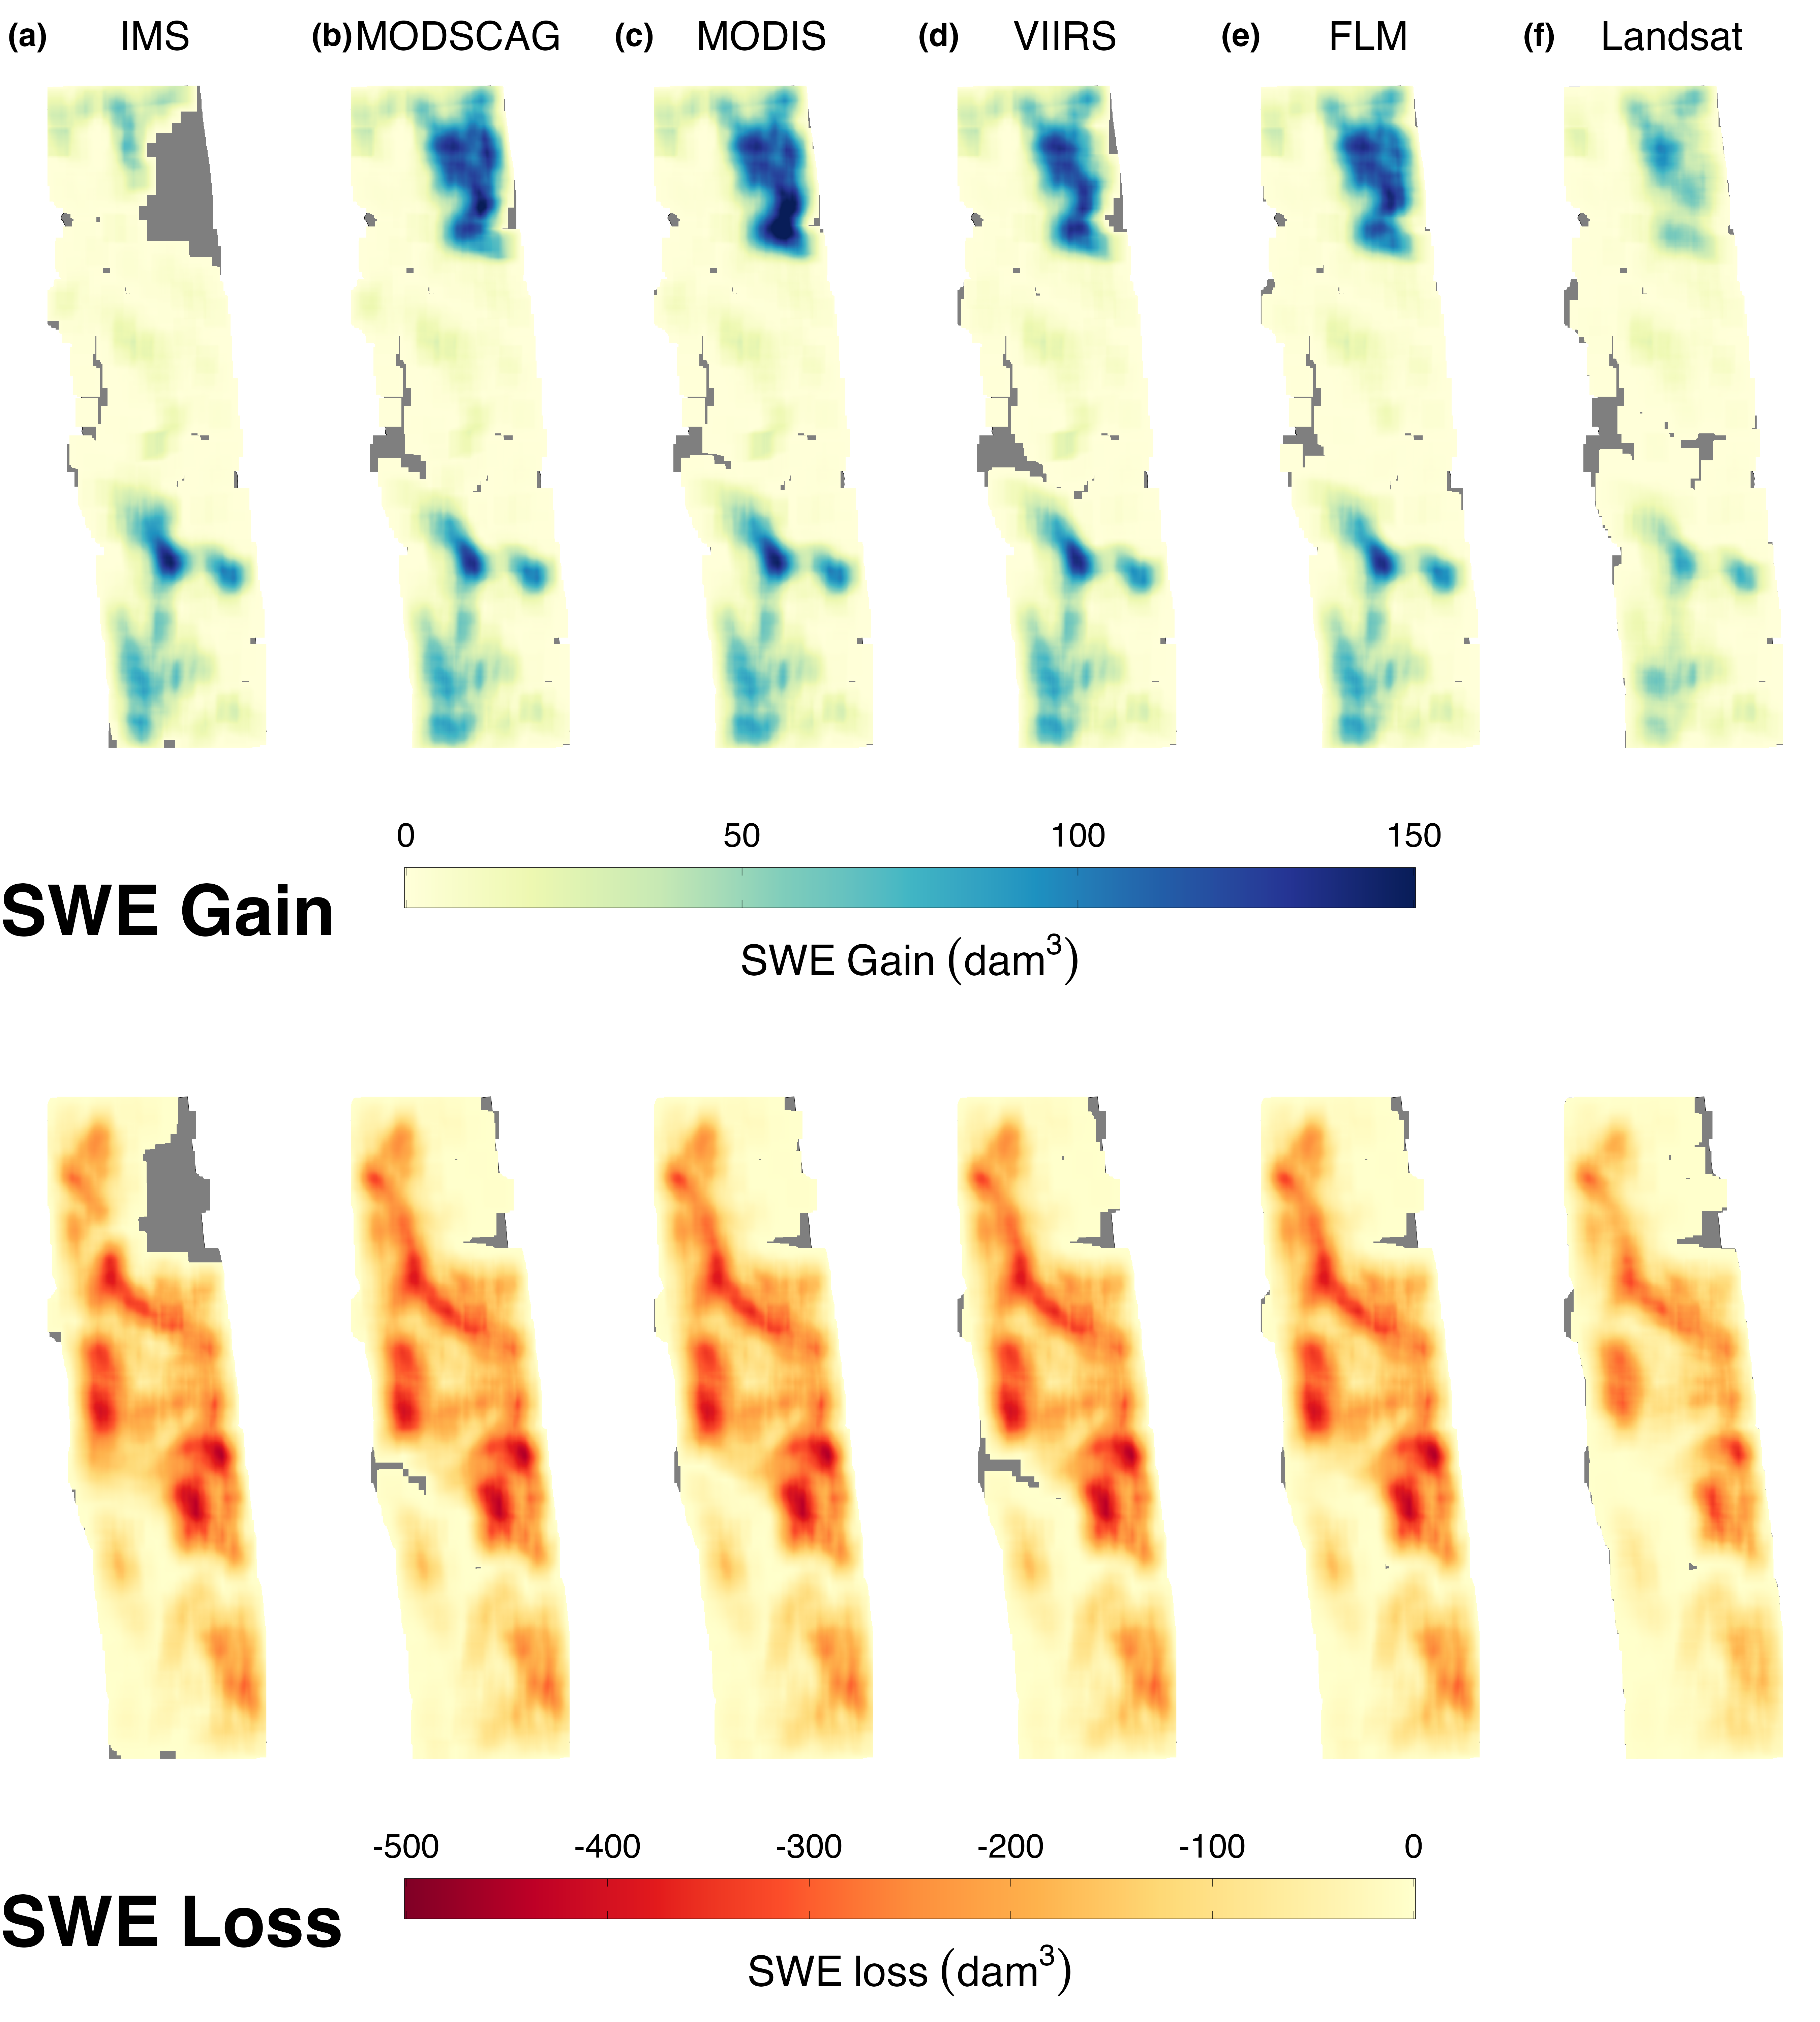
\includegraphics[width=\textwidth]{figures/ch4_figs/dswe_mw_full_dam3_v1.png}
\caption{$\Delta$SWE moving window analysis for SWE gains (top) and SWE losses (bottom) for the six different $\Delta$SWE products.}
\label{fig:dswe_moving_window}
\end{figure}


\clearpage
\begin{figure}[t]
\centering
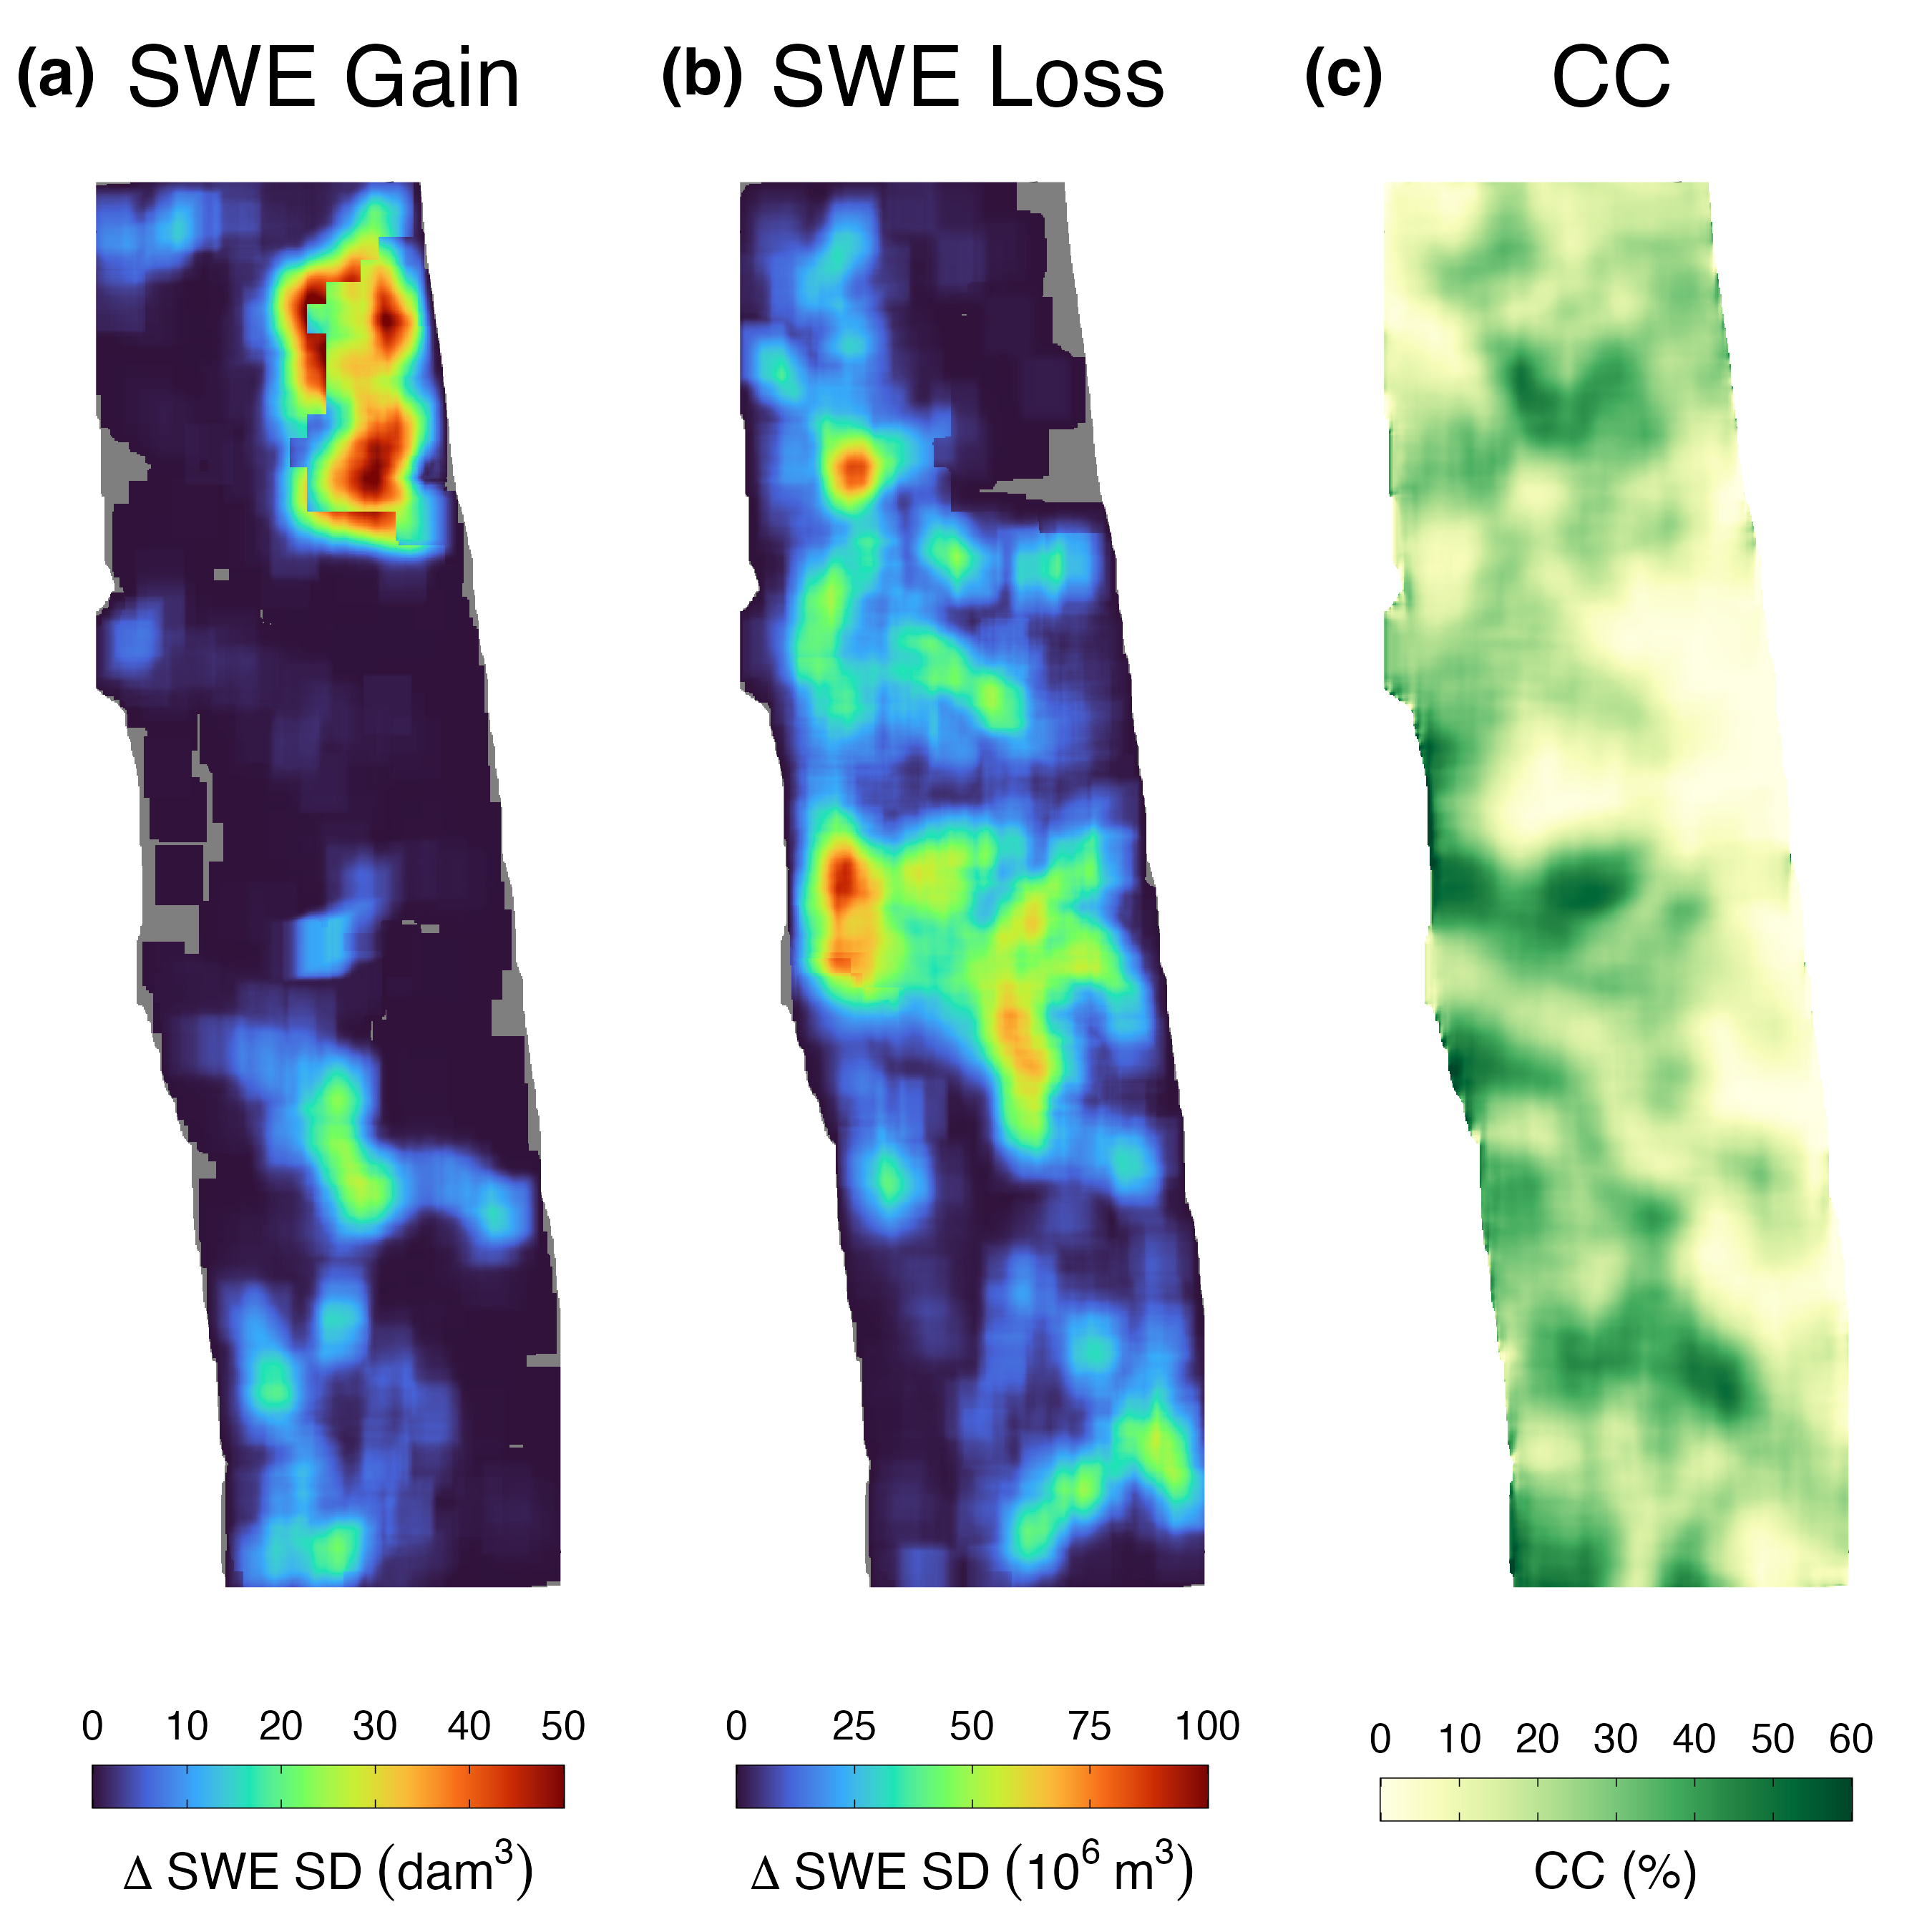
\includegraphics[width=\textwidth]{figures/ch4_figs/sd_vs_cc_map_dam3_41x41.png}
\caption{***FIX UNITS**** Showing SD \textbf{(a)} SWE gain and \textbf{(b)} SWE Loss between the six a 41~$\times$~41 pixel moving window $\Delta$SWE estimates. \textbf{(c)} The moving window canopy cover percentage.}
\label{fig:dswe_standard_deviation}
\end{figure}

\clearpage
\begin{figure}[t]
\centering
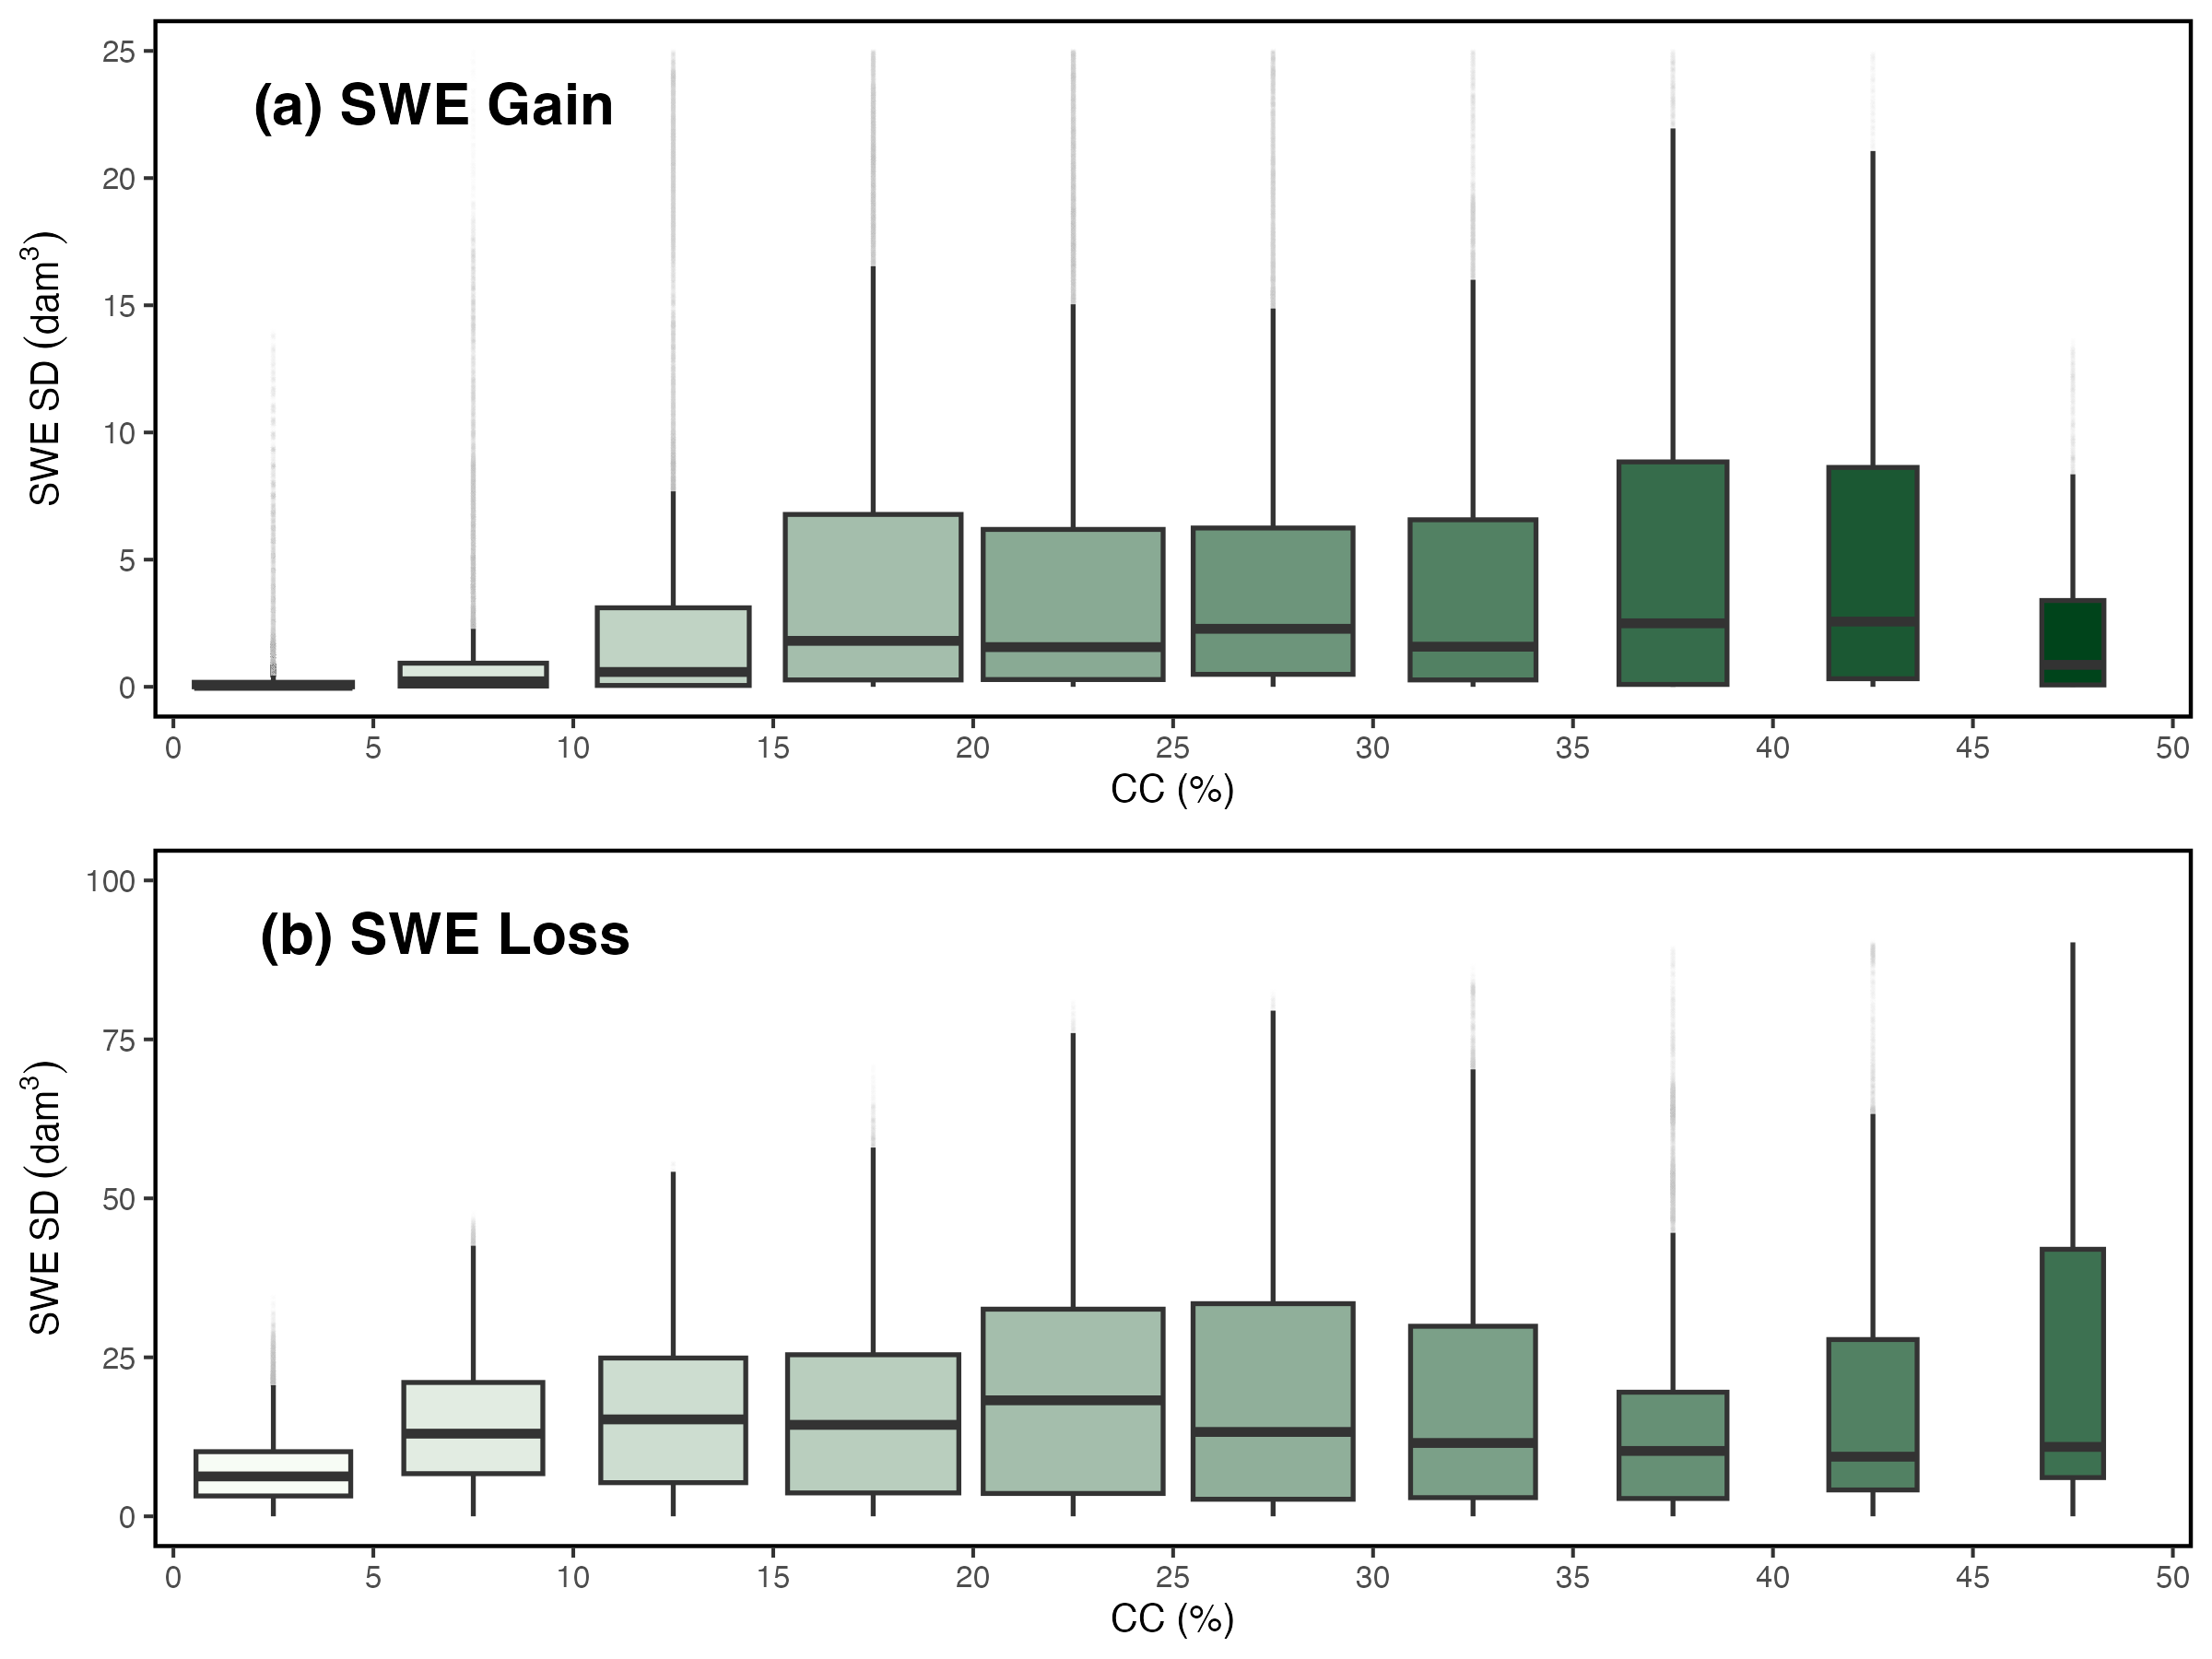
\includegraphics[width=\textwidth]{figures/ch4_figs/swe_sd_bp_dam3_41x41_v1.png}
\caption{Boxplots showing the relationship between CC \% and SWE SD for \textbf{(a)} gain and \textbf{(b)} loss. The y-axis is set individually for each plot for data visualization purposes.}
\label{fig:dswe_boxplots}
\end{figure}






%==============================================================================
%==============================================================================
%==============================================================================
\hypertarget{ch5-discussion}{\section{Discussion}\label{ch4-discussion}}
\hypertarget{ch5-discussion-1}{\subsection{Key findings and future directions}\label{ch4-discussion}}

We ***originally hypothesized*** FLM would provide the most realistic results as it uses information from both Landsat and MODIS. While the coarser native resolution values of MODIS and MODSCAG (500~m) and VIIRS (375~m) create blocky results around the snowline, these differences don't significantly impact the overall $\Delta$SWE results when compared to FLM. \cite{stillingerLandsatMODISVIIRS2023a} performed an uncertainty analysis of various fSCA products from MODIS, VIIRS, and Landsat using airborne lidar-based fSCA as validation. They found some variability in the fSCA products, with the spectrally unmixed data performing better, but overall modest differences. It is promising that fSCA derived from MODIS and VIIRS NDSI data, currently produced in near-real-time by NSIDC, can generate fSCA estimates for SAR-based SWE retrievals that yield nearly identical values (\ref{tab:dswe_stats}) to that of the more complex spectral unmixing and machine learning methods employed by MODSCAG and FLM. Additionally, these products are not currently hosted openly on a NASA DAAC. This means that upon the launch of NISAR in early 2024, the moderate-resolution sensor can provide a reasonable snow cover boundary for basin-scale water resource applications. 

While there were broad similarities, our results show that significant InSAR-based $\Delta$SWE estimation variability can arise from fSCA product choice. The variability in how snow cover is defined arises from two main sources: primarily sub-canopy snow cover estimation methodology and secondarily native product spatial resolution. The five fSCA products, excluding Landsat, showed broad similarities in their fSCA estimation in forest areas. For the coarser resolution products (MODIS, VIIRS, IMS), the larger pixel size has more sub-pixel variably, with fewer pixels having less than 15~\% fSCA. For the finer-resolution products (FLM and Landsat), their main differences arise from the sub-canopy fSCA estimation. The Landsat fSCA data had the greatest differences in fSCA, which then propagated into SWE gains and losses of lesser magnitude when compared to the other five products. These losses are driven by how the Landsat data estimate sub-canopy snow cover. They use a multi-step moving window canopy adjustment. It employs a 11~$\times$~11 and a 31~$\times$~31 moving window to the infill surrounding pixels depending on NLCD canopy cover percentage, elevation, cloud cover, and solar radiation \citep{selkowitzUSGSLandsatSnow2017}. If a pixel is >~60~\% canopy cover, it is automatically excluded from snow cover eligibility. We hypothesize that the dense conifer forest in parts of the UAVSAR study area, with 48~\% of the total forest having a canopy cover density of >~40~\%, created conditions where the algorithm didn't detect sub-canopy snow cover. As noted in \cite{bairHowTradeoffsSatellite2023}, the discretization of the study area (i.e., the amount of land area considered inside the study area) is inherently different depending on the native product resolution. This impacted the snow line estimates but was of lesser concern when compared to the canopy cover considerations.

%%% thoughts on fSCA and forests
It is important to note that fSCA data has not traditionally been used in combination with radar data for SWE estimation. Past SWE estimation work has implemented fSCA in combination with a spatially distributed energy balance model to derive SWE in various reconstruction approaches \citep{clineEstimatingSpatialDistribution1998,molotchEstimatingDistributionSnow2008,rittgerSpatialEstimatesSnow2016,margulisLandsatEraSierraNevada2016}. **We employed a 15\% fSCA threshold to determine the inclusion of pixels as snow-covered. This is a subjective choice based on the minimum threshold set in \cite{painterRetrievalSubpixelSnow2009}. While not the main focus of this study, future work should focus on the uncertainties associated with all SAR-based SWE retrievals techniques fSCA and canopy cover. Whether it's the InSAR phase-based technique presented here with L-band, P-band \citep{shahRemoteSensingSnow2017,maEstimatingSpatiotemporallyContinuous2023}, C-band \citep{lievensSnowDepthVariability2019,oveisgharanSnowWaterEquivalent2023}, or Ku-band \citep{tsangReviewArticleGlobal2022,rottColdRegionsHydrology2010}, all techniques will have to quantify the uncertainty associated with mixed pixels. As seen the in the Landsat fSCA data used in this study, very few 80~m square areas are completely snow-covered. There are bare areas driven by prevailing wind patterns and aspect-based solar radiation variations, as well at large areas of the swath consistent conifer forest canopy. In the Cold Regions Hydrology High-Resolution Observatory (CoReH$_{2}$O) mission (Ku-band) developed by \cite{rottColdRegionsHydrology2010}, they note the importance of accounting for three-dimensional canopy structure on backscatter values. \cite{lemmetyinenAttenuationRadarSignal2022} showed radar signals at various wavelengths have different sensitives to forest canopy, with above-freezing temperatures increasing the uncertainty. Continuing to unravel the impacts of forests on SAR-based SWE retrievals from airborne and spaceborne platforms should be the topic of future investigations.


%%%%%%%%%%%%%%%%%%%%%%%%%%%%%%%%%%%%%%%%%%%%%%%%%%%%%%%%%%%%%%%%%%%%%%%%
%%%%%%%%%%%%%%%%%%%%%%%%%%%%%%%%%%%%%%%%%%%%%%%%%%%%%%%%%%%%%%%%%%%%%%%%
%%%%%%%%%%%%%%%%%%%%%%%%%%%%%%%%%%%%%%%%%%%%%%%%%%%%%%%%%%%%%%%%%%%%%%%%
\hypertarget{ch5-discussion-2}{\subsection{Limitations and Future Work}\label{ch4-discussion-2}}

% no truth, just variability
Our study did not aim to validate the given data products with respect to validation dataset. Many past studies have used Landsat, with various spectral unmixing approaches, as their validation data set \citep{painterRetrievalSubpixelSnow2009,rittgerAssessmentMethodsMapping2013 } or airborne lidar \citep{stillingerLandsatMODISVIIRS2023a}. While it's impossible to confidently say whether or not a sub-canopy area is completely snow covered, we assume that the high-elevation parts of the USJ were snow covered. This suggests that Landsat was underestimating fSCA and $\Delta$, as it had far greater amount of pixels considered NA.

% study area and short time period
The UAVSAR flight line was over a high elevation (mean of 2733~m) portion of the USJ, where a majority of the swath was snow covered. During the two-week study period, there were no large precipitation events, and therefore snow cover was relatively constant. In future satellite-based full basin-scale analyses, there will be a greater range and variability of fSCA values, as well as more lower-elevation forest cover. Additionally, large atmospheric river-type storms in the Sierra can significantly shift the snow line. This presents challenges for the products that are daily, such as Landsat. We chose to analyze data over a short study window (12~d) and therefore did not fully address the effects temporal resolution has on SWE change estimates. Future work should focus on the $\Delta$SWE uncertainties that come from infrequent fSCA data.

% swe change tie point and density uncertanities
We used an average SWE change between three snow pillows to set the InSAR known change point. As seen in **Appendix Table 1, there was disagreement between the UAVSAR predict SWE change and the in situ values. 


However, future work should continue to focus estimate fSCA at finer spatial resolutions. The incorporation Very-High-Resolution (VHR) commercial satellite imagery: sources are \citep{huImprovingMountainSnow2022, thalerEstimatingSnowCover2023,yangHighresolutionMappingSnow2023,johnHighResolutionSnowCoveredArea2022}


-Our variability analysis was an imperfect comparison between the six data products. While we used a 41 $\times$ 41 moving window, the IMS data had a large continuous snow free area in the northeast corner. These pixels were then omitted from the standard deviation analysis, propagating uncertainty in the calculation as one dataset was not used.

However, future work should continue to focus estimate fSCA at finer spatial resolutions. The incorporation Very-High-Resolution (VHR) commercial satellite imagery: sources are \citep{huImprovingMountainSnow2022, thalerEstimatingSnowCover2023,yangHighresolutionMappingSnow2023,johnHighResolutionSnowCoveredArea2022}


%==============================================================================
%==============================================================================
%==============================================================================
\hypertarget{ch6-conclusions}{\section{Conclusions}\label{ch6-conclusions}}

This study set out to understand how fSCA product selection impacts $\Delta$SWE estimates in a multisensor optical-radar approach. While 


\clearpage
\bibliographystyle{apalike}
\setstretch{1}
\bibliography{ch4.bib}
\setstretch{1.5}
